\chapter{Design and Implementation of the Forwarding Strategy by MAC Addresses}

The main goal of this thesis is to extend the current ndnSIM 2.0 implementation in order to allow efficient communication between mobile agents. A first interest packet is broadcast by the consumer on one channel and forwarded by all intermediate nodes in a broadcast manner. Default routes are set by the NFD at the beginning and need to be overridden as soon as more information is obtained. After being forwarded by the intermediate nodes the Interest arrives at the producer and a corresponding Data packet is created. This packet returns to the consumer and will add routes by updating the FIB entries.

\section{Problem Description}

The current implementation relies only on face ids of the application or net device (\texttt{ndn::NetDevice}), which is sufficient for point to point connections but will not work on wireless communication like in the mobile ad-hoc scenarios investigated in this thesis. All examples found so far use a point to point topology, where wires connect different faces of different nodes. Sending an Interest to one face defines automatically on which face and node the Interest will arrive. A path exists and is uniquely identified by the combination of node and face. If several net devices exist on a node, their face id will be assigned incrementally starting from the id 256 resulting in faces with the same id. Wireless communication is inherently broadcasting and the nodes are responsible for accepting the packet if it was meant for them and drop it if it was only overheard. On wireless communication sending a message through a face results in broadcasting the message, and therefore a specific route cannot exist, by defining only the out-face of the node, obtained from the FIB entry. The same goes for data being forwarded through faces downstream towards a consumer. The topology is not known and changing fast so there needs to be a way to identify specific nodes in a consistent manner.

If one route is found and the FIB entries have been updated, Interests will follow this path to the producer and data will follow the breadcrumbs back to the consumer. That will likely lead to congestions and incur unnecessary overhead on some of the intermediate nodes. Other nodes are potentially left out all together since no FIB entries are configured to point to them. Having the possibility to chose from different channels and different paths will spread the load onto different intermediate nodes making congestions and retransmissions less likely.

This thesis focuses on a new forwarding strategy for vehicular ad-hoc networks. In the two distinct scenarios, only one consumer and one producer are used and the consumer requests different data every time. A content store caches data for later use if another consumer happens to request the very same data. Since this thesis does not implement several consumers requesting the same information, no content store has been implemented. Returning data is not cached in intermediate nodes for later use. If more consumers are introduced to the scenario, a content store implementation should not be missing.


\section{Multipath Approach}

In order to support paths, the nodes must know where the packet did come from and where to forward it to. ndnSIM's default installation solves this issue through faces, which are attached to the net devices of the nodes. The faces of the net device cannot be used since they are equal on each node. Numbers starting from 256 are assigned to the faces as ids in an incrementing order and if there are 10 nodes in the network there will be 10 faces with the same face id of 256. Also, the application faces will be the same on the consumer and the producer. In order to solve this problem, a new identifier needs to be found that can identify each node. Net devices are required for any kind of inter-node connections and they have unique MAC addresses, which are set at the beginning for every simulation and will not clash with other net devices. Therefore, they make a perfect substitution for the current faces used for point to point configurations and can be used in WiFi scenarios. Net Devices are implemented in ndnSIM through the \texttt{ndn::NetDevice} class.

\subsection{Changes to the Interest Message}

In order to populate the FIB entries, the information about the topology must be communicated to all surrounding neighbors. The information about previous nodes that have been encountered, while forwarding the Interest towards a potential content source, can be added to the Interest. That makes it possible to forward the data downstream towards the requester by following the breadcrumbs left in the PIT entries. These breadcrumbs consist in our implementation of the MAC addresses of the net device from the previous node. The Interest has three new fields:

\clearpage

\begin{itemize}
\item \emph{std::string m\_interestOriginMacAddress}: This field has the MAC address of the previous node.
\item \emph{std::string m\_interestTargetMacAddress}: This field has the MAC address of the next node, that the Interest should be forwarded to. It is possible that the FIB entry exists but no MAC address is configured yet.
\item \emph{std::string m\_macInterestRoute}: This field shows the the way of the Interest so far.
\end{itemize}

The following figure \ref{fig:incomingInterestPipelineWithMac} illustrated the MAC address relevant steps in the incoming Interest pipeline \texttt{Forwarder::onIncomingInterest}.

\vspace{5mm} %5mm vertical space

\begin{figure}[H]
  \centering
  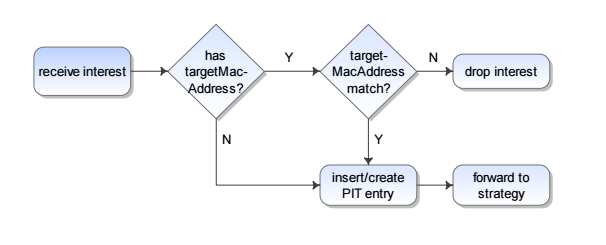
\includegraphics[scale=0.6]{chapter-4/incomingInterestPipelineWithMac}
  \caption{Incoming Interest pipeline for the implementation of MAC addresses}
  \label{fig:incomingInterestPipelineWithMac}
\end{figure}

\vspace{5mm} %5mm vertical space

At the beginning of the simulation, no knowledge about the topology is present. The first Interest is broadcast. Since the FIB entries have not yet been populated with information on neighboring nodes and their MAC address, the first Interest cannot have a valid targetMacAddress. The missing MAC address signals to all receiving nodes that the Interest is being flooded through the network and needs to be broadcast further. After information about the topology is present the Interest will have a valid MAC address of the target it is supposed to reach.

When a node receives an Interest either from another node or from an application, the following steps (from figure \ref{fig:incomingInterestPipelineWithMac}) are performed:

\begin{enumerate}
\item The \emph{Interest::m\_interestTargetMacAddress} is checked for a valid MAC address through regular expressions.
\item If the Interest has no valid target MAC address the Interest is accepted as being broadcast. It will be inserted into the PIT table with it's attached origin MAC address. The origin MAC address tells the node where the Interest came from and will be used later for the Data to be forwarded downstream towards the content requester.
\item If a valid MAC address was found, it is checked against the receiving net device's MAC address.
\item If the Interest's target MAC address equals the receiving net device's MAC address the Interest was meant for this node (in particular for this net device) and will be inserted into the PIT table with its origin MAC address. If the two MAC addresses (target MAC address and the current device's MAC address) do not match, the Interest was not meant for this node and will be dropped immediately to save resources. No overhearing occurs at any time with the Interest. Interests are only forwarded to specific nodes or broadcast.
\item The Interest will be forwarded to the strategy for further processing.
\end{enumerate}

All Interests have valid \emph{std::string m\_interestOriginMacAddress} fields at all time. These are needed to leave the breadcrumbs for the returning data and are inserted into the PIT entries at the time of arriving at a new node. If the incoming Interest had a valid target MAC address, it will be checked if it matches any MAC address on the node. In that case, the target MAC address will become the outgoing Interest origin MAC address, since it will be leaving this node through the current net device it was originally received on. If no valid target MAC was given to the incoming Interest a new current MAC address must be chosen from all active net devices on this node. This is done through a static counter and the modulo expression, making sure, that different paths are taken. Adding the new origin MAC address happens in \texttt{Forwarder::onOutgoingInterest} or in \texttt{Strategy::afterReceiveInterest}.

\subsection{Changes to the Data Message}

In order to have routes and the FIB entries populated, the information about the topology must be communicated to all the surrounding neighbors. The data is responsible for populating the FIB entries with new MAC addresses from nodes further upstream. The data carries that information, which is the MAC address of the previous node the data was forwarded from. Existing FIB entries can be updated or new routes can be added with the help of the \texttt{ns3::ndn::FibHelper} helper class by calling the \texttt(AddRoute) method.

The Data object is also extended with three new member variables:

\begin{itemize}
\item \emph{std::string m\_dataOriginMacAddress}: This field has the MAC address of the previous node.
\item \emph{std::string m\_dataTargetMacAddress}: This field has the MAC address of the next node if a MAC address was left in the PIT entry.
\item \emph{std::string m\_macDataRoute}: This field shows the way of the Data message so far.
\end{itemize}

The following figure \ref{fig:incomingDataPipelineWithMac} illustrates the MAC address relevant steps in the incoming data pipeline \texttt{Forwarder::onIncomingData}.

\vspace{5mm} %5mm vertical space

\begin{figure}[H]
  \centering
  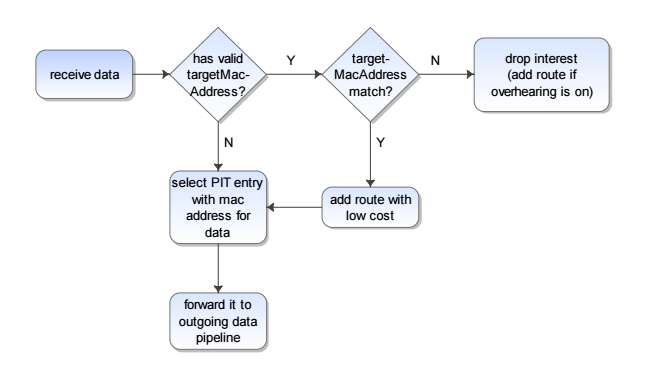
\includegraphics[scale=0.6]{chapter-4/incomingDataPipelineWithMac}
  \caption{Incoming data pipeline for Data messages}
  \label{fig:incomingDataPipelineWithMac}
\end{figure}

\vspace{5mm} %5mm vertical space

The steps are explained as follows:

\begin{enumerate}
\item After the node has received the Data packet, the member variable  \emph{Data::m\_dataTargetMacAddress} is checked for a valid MAC address through regular expressions.
\item If the target MAC address of the Data is equal to the current net device's MAC address the Data was meant for this node. If the MAC addresses do not match, the Data was overheard.
\item It depends on the implementation if overheard Data shall be further processed, cached into CS or just dropped. The overheard Data can also be used to populate FIB entries, in order to obtain more routes for the Interests, but not be saved into CS.
\item If the Data was intended to be received by this node, a route is added through the \texttt{ns3::ndn::FibHelper::AddRoute} helper method. The cost of this new next hop needs to be set lower than for default next hop or the next hops resulting from overheard Data. This is important, because the FIB entries are sorted by cost in ascending fashion.
\item From the corresponding PIT entry (retrieved by longest prefix match) the downstream MAC address and face information are retrieved and then added to a copy of the Data. The copy is needed since the Data is defined as constant.
\item The updated copy of the Data is then handed off to the outgoing data pipeline.
\end{enumerate}

The outgoing data pipeline is implemented in \texttt{Forwarder::onOutgoingData}. It receives the Data with additional parameters. If the target MAC address of the Data is valid and the Data is solicited, the origin MAC address field of the Data is updated with the MAC address of the current net device responsible for forwarding this Data. If the Data was unsolicited a new MAC address of the possible net devices is selected in an alternating manner and added to the Data. The route is updated and the Data is sent through it's out-face to the next node.

The data encoding of the Interest and Data packets had to be extended by the new fields in order to be sent over the network and to be received by other nodes.

\subsection{Changes to the FIB}

The FIB entries hold information about how to forward the Interest upstream. Every FIB entry is uniquely identified by the prefix of the incoming Interest. It is found by longest prefix match. The entry aggregates NextHop objects with the corresponding faces and cost information as shown in chapter 3 figure \ref{fig:FIBdataStructure}.
In this thesis, forwarding is not done by faces as initially implemented in ndnSIM \cite{Afanasyev16}, but by MAC addresses. These MAC addresses are updated inside existing FIB entries or new FIB entries are created with this additional information. Therefore the new FIB entries have been extended with functions to fetch the new information from the NextHop entries. And the NextHop entries have been extended by a new MAC address field.

\vspace{5mm} %5mm vertical space

\begin{figure}[H]
  \centering
  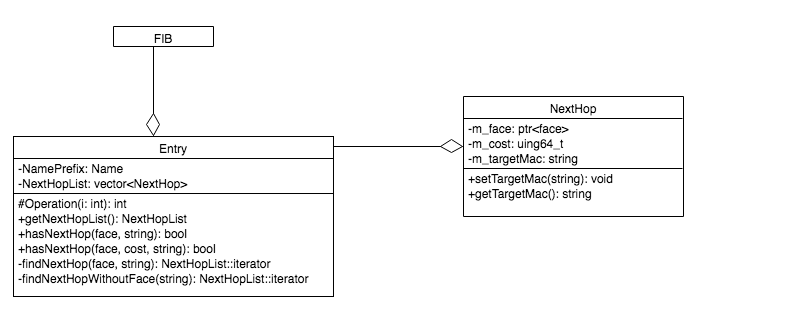
\includegraphics[scale=0.6]{chapter-4/newFIBdataStructure}
  \caption{FIB new Data structure}
  \label{fig:newFIBdataStructure}
\end{figure}

\vspace{5mm} %5mm vertical space

Figure \ref{fig:FIBdataStructure} shows only the relevant and new member variables and methods added to the Data structure. The FIB entries need new methods that find next hops according to the MAC addresses or a combination of MAC addresses and faces. A new method returns a NextHopList that is passed by reference. The NextHop class has been extended by the target MAC field, setters and getters.

\newpage

\subsection{Changes to the PIT}

The PIT entries hold information about how to forward the data downstream. Every PIT entry is uniquely identified by the prefix of the incoming Data. It is found by longest prefix match. The entry aggregates in-record and out-record objects with the corresponding faces, lastNonce and lastRenewed information, as shown in chapter 3 figure \ref{fig:PITdataStructure}. The faces need to be extended by MAC addresses since the data is broadcast and the receiving node needs to identify if it is the intended recipient.

\vspace{5mm} %5mm vertical space

\begin{figure}[H]
  \centering
  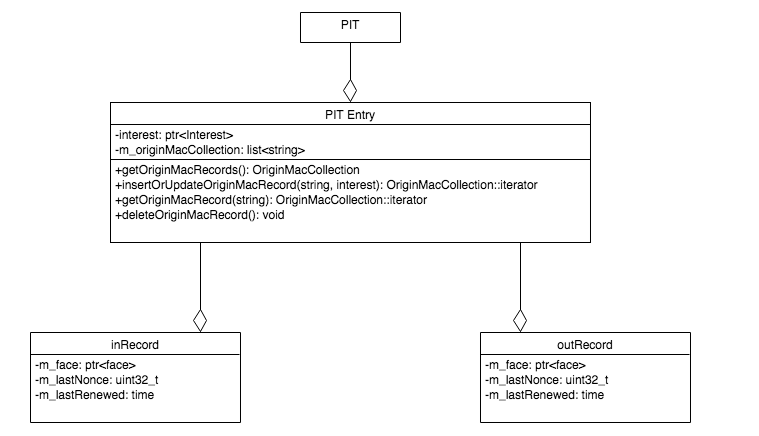
\includegraphics[scale=0.6]{chapter-4/newPITdataStructure}
  \caption{New PIT Data structure}
  \label{fig:newPITdataStructure}
\end{figure}

\vspace{5mm} %5mm vertical space

Figure \ref{fig:newPITdataStructure} shows only the relevant and new member variables and methods added to the Data structure. A new list member variable \texttt{m\_originMacCollection} has been added to the PIT entry. Every Interest forwarded correctly leaves it's origin MAC address in this list. When requested data arrives at the node, the origin MAC collection in the PIT entry is checked and attached to the Data's field. Methods, setters and getters encapsulate the member variable within its class.





